\documentclass[12pt,a4paper]{article}
\usepackage{color}
\usepackage{parskip}% http://ctan.org/pkg/parskip
\usepackage{graphicx} 
\usepackage{hyperref}

% \setlength{\parindent}{0pt}

\title{IBSimu Particle Diagnostic \\
	\large Working Draft}
\date{2020-11-30}
\author{Duccio Marco Gasparri}

\begin{document}
  \maketitle
  
\section{variables}
\begin{itemize}
	\item m [kg] particle mass (provided in u)
	\item q [J] charge of beam particle (provided in multiples of e)
	\item J [A/m\^2] beam current density
	\item E [J]  mean energy (provided in eV)
	\item Tp [J] parallel temperature (provided in eV)
	\item Tt [J] transverse temperature (provided in eV)
	\item ($x_{1}, r_{1}), (x_{2}, r_{2}$) [m] beam emission line vectors
	\item N number of particles
	\item IQ [A] (A/m?) particle current
	\item v [m/s] from E and m
\end{itemize}

\section{Setup}
\subsection{Geometry}

Relevant IBSimu files:
\begin{itemize}
	\item geometry.hpp 
	\item geometry.cpp
	\item mesh.hpp
	\item mesh.cpp
\end{itemize}



Relevant client files:
\begin{itemize}
	\item configuration-setup.hpp
	\item configuration-setup.cpp
\end{itemize}


Parameters:
\begin{itemize}
	\item mesh-cell-size-h [eg. 0.5e-4]
	\item origin-x 
	\item origin-y
	\item origin-z
	\item geometry-start-x [UNUSED]
	\item geometry-start-y [UNUSED]
	\item geometry-start-z [UNUSED]
	\item geometry-size-x
	\item geometry-size-y
	\item geometry-size-z
\end{itemize}

The class Geometry creates the mesh of the simulation starting from the CAD files and/or function definitions.

The parameters origin-x, origin-y and origin-z are used to move the reference frame relative to the bbox in the DXF file [see mesh.hpp line 70-73, mesh.cpp line 60].


\begin{figure}
	\centering
	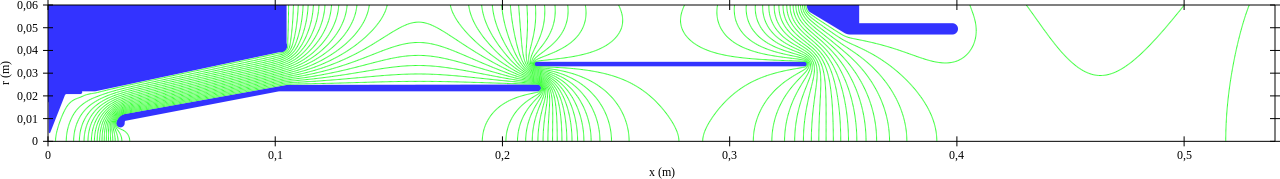
\includegraphics[width=0.7\linewidth]{"assets/geometry_origin_x_zero.png"}
	\caption[Origin X = 0]{Geometry DXF starting at -10e-3 m. Setting origin-x = 0 mm}
	\label{fig:esempio-origin-xzero}
\end{figure}

\begin{figure}
	\centering
	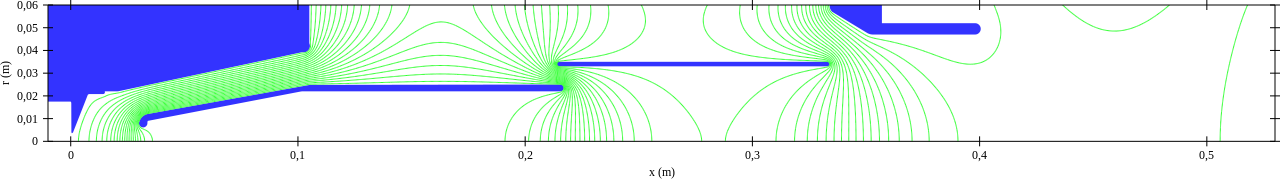
\includegraphics[width=0.7\linewidth]{"assets/geometry_origin_x_minus10mm.png"}
	\caption[Origin X = 0]{Geometry DXF starting at -10e-3 m. Setting origin-x = -10 mm}
	\label{fig:esempio-origin-xzero}
\end{figure}


IBSimu does not render the space before the origin-x, so also moving the geomtery with the mouse would not show the part before the origin-x.

NB: Non si capisce perché non calcoli il campo elettrico prima dello zero della geometria. Avevo la geometria traslata a -10mm, con zero la punta dell'elettrodo di estrazione. Tra [-10mm;0] l'epot era = a Vplasma



The physical length/height/depth of the simulation is size-x/y/z * mesh-cell-size. Specifically:

$$size-x = (int)floor(geometry-size-x / mesh-cell-size-h) + 1 $$
$$x_{max} = origin-x + mesh-cell-size-h * size-x$$







\section{ParticleDataBaseCylImp::add\_2d\_beam\_with\_energy}

Function ParticleDataBaseCylImp::add\_2d\_beam\_with\_energy (file: \textit{particledatabaseimp.cpp}, line: 968) is used to add a beam of N particles with average energy E to a cylindrical geometry.

The charge q is provided by the user and is set constant for all the particles.

The beam emission line norm s [m] is defined:

\begin{equation}
	s = \sqrt{(x_{2}-x_{1})^2+(r_{2}-r_{1})^2}
\end{equation}

The current IQ [A] is set for each particle as follows:

\begin{equation}
	IQ =\frac{2\pi sJ}{N}(r_{1} + \frac{(r_{2}-r_{1})}{N}(n+0.5))
\end{equation}

where $n\in[0,1,...,N-1]$. 

The particles are distributed evenly spaced along the emission line defined by the vectors $(x_{1},r_{1}), (x_{2},r_{2})$. The particle velocities $v_{x},v_{r}$ [m/s] are:

\begin{equation}
	v_{x}=\frac{(x_{2}-x_{1})}{s}\sqrt{\frac{Tt}{m}}rnd_{0}+\frac{(r_{2}-r_{1})}{s}\sqrt{\frac{2E}{m}+(\sqrt{\frac{Tp}{m}}rnd_{1})^2}
\end{equation}

\begin{equation}
	v_{r}=\frac{(r_{2}-r_{1})}{s}\sqrt{\frac{Tt}{m}}rnd_{0}+\frac{-(x_{2}-x_{1})}{s}\sqrt{\frac{2E}{m}+(\sqrt{\frac{Tp}{m}}rnd_{1})^2} 
\end{equation}

and

\begin{equation}
	w=\frac{d\theta}{dt}=\frac{\sqrt{\frac{Tt}{m}}rnd_{2}}{r_{1} + \frac{(r_{2}-r_{1})}{N}(n+0.5)}
\end{equation}

with $rnd_{0}$, $rnd_{1}$ and $rnd_{2}$ normally distributed random variables.


\section{Iteration}

The method ParticleDataBasePPImp::iterate\_trajectories (inherits ParticleDataBaseImp, file: particledatabaseimp.hpp::641) outputs the message "Using non-relativistic iterator", clears the scharge, creates a iterators vector of size equal to the set thread, populates it with new instances of ParticleIterator<  PP>  and waits for the iteration to be finished. Then calls scharge\_finalize\_linear (file:scharge.cpp:149) Finally it publishes the particle hisories ("Particle histories").

scharge\_finalize\_liear prints "Finalizing space charge density map (LINEAR method)"

The core of the iteration isinside the ParticleIterator<PP>



The method ParticleDataBasePPImp::iterate\_trajectories (inherits ParticleDataBaseImp, file: particledatabaseimp.hpp::641) outputs the message "Using non-relativistic iterator", clears the scharge, creates a iterators vector of size equal to the set thread, populates it with new instances of ParticleIterator<PP> and waits for the iteration to be finished. Then calls scharge\_finalize\_linear (file:scharge.cpp:149) Finally it publishes the particle hisories ("Particle histories").

scharge\_finalize\_liear prints "Finalizing space charge density map (LINEAR method)"

The core of the iteration isinside the ParticleIterator<PP>


Scheduler class 

Scheduler is templated with Solver, Problem and Error classes. 

From ParticleDatabasePPImp (particledatabaseimp.hpp:291):

std::vector<Particle<PP> *>                        \_particles;
Scheduler<ParticleIterator<PP> (as Solver), Particle<PP> (as Problem), Error (as Error)> \_scheduler;



Scheduler class requires the Solver class ParticleIterator<PP> to provide an operator

  void ParticleIterator<PP>::operator()( Problem *p, int32\_t pi )

or, as implemented, Problem is Particle<PP>

 void ParticleIterator<PP>::operator()(Particle<PP> *particle, uint32\_t pi)
  
to solve problem p with index location pi. (particleiterator.hpp:1258)

The operator calls the PP::get\_derivatives( 0.0, \&x[1], dxdt, (void *)\&\_pidata ); function to 
fill dxdt (particleiterator.hpp:1298).

double dxdt[PP::size()-1];

For the ParticlePCyl::get\_derivatives(...) function, documentation reports:

"Returns time derivatives dxdt of coordinates at time t and coordinates x = (x,vx,r,vr,w) for one particle.

The calculation of particle trajectory is done by integrating the Lorentz equation in a form of a set of ordinary differential equations. In the case of cylindrical coordinates the set is:

$$\frac{dx}{dt} = v_{x}$$

$$\frac{dr}{dt} = v_{r}$$

$$\frac{dv_{x}}{dt} = a_{x} = \frac{q}{m}(E_{x}+v_{r}B_{\theta}-v_{\theta}B_{r})$$

$$\frac{dv_{r}}{dt} = a_{r} + r\left ( \frac{d\theta}{d}\right )^{2} = \frac{q}{m}(E_{y}+v_{\theta}B{x}-v_{x}B_{\theta})+r\left ( \frac{d\theta}{d}\right )^{2}$$

$$\frac{d^{2}\theta}{dt^2} = \frac{1}{r}\left(a_{\theta}-\frac{dr}{dt}\frac{d\theta}{dt}\right) =
 \frac{1}{r}\left(\frac{q}{m}(v_{x}B_{r}-v_{r}B_{x}) -2\frac{dr}{dt}\frac{d\theta}{dt}\right)
$$

where 

$$v_{\theta} = r\frac{d\theta}{dt}$$

End quote. Source: \url{http://ibsimu.sourceforge.net/manual_1_0_6/classParticlePCyl.html#adb44dff844a1af2615727a1920c18c8b}


, then 

double dt = ParticleIterator<PP>calculate\_dt( x, dxdt );

to get initial dt.



Then the GSL odeiv functions are called to advance the particle, and the result is checked with the ParticleIterator<PP>::handle\_trajectory() function (particleiterator.hpp:1361)

The bool ParticleIterator<PP>::handle\_trajectory() function searches mesh intersections between points x1 and x2 and builds ColData. Checks for collisions with solids and boundaries and sets space charge at each mesh line crossing.


Error class has to have a default constructor. Scheduler catches
the errors of this type from the working threads and saves caught
errors in a container. If an error is caught, all the working
threads are interrupted and problem solving is finished. The
scheduler does indicate the error state by returning false from
finish(). Error state can also be queried with is\_error(). Errors
can be fetched from the internal containers with get\_errors().
The %Scheduler can be used for static and dynamic problems. All
threads can add problems. The problem vector is a shared resource
so it must be protected with lock\_mutex() and unlock\_mutex().

Parallel processing is started with run() function and the end of
processing can be waited with finish().






\section{Particle Diagnostic}

The relevant functions are in files gtkparticlediagdialog.cpp (the GTK dialog file) and particlediagplot.cpp (does the actual plotting). It has the following methods:

\begin{itemize}
	\item ParticleDiagPlot::build\_data(): the function extracts the data from the ParticleDatabase
	\item ParticleDiagPlot::build\_plot(): calls build\_data(). the function extracts the data from the ParticleDatabase, set the decorations and add the graph to the \_frame
\end{itemize}


Trajectories are obtained from ParticleDataBase::trajectories\_at\_plane() that calls ParticleDataBaseImp::trajectories\_at\_plane(). It requires the axis (X, Y, Z, R) and the distance from origin. It returns a vector of particle point objects ParticleP<PP> (either ParticleP2D, ParticlePCyl, or ParticleP3D), each particle carrying its information about position and momentum

q is the direction normal to the diagnostic plane

DIAG\_X: x position [m]
DIAG\_R: r position [m]



DIAG\_RP: $\frac{v_r}{v_q}$

DIAG\_AP: $\frac{v_\theta}{v_q}$

$$v_\theta=r\frac{d\theta}{dt}$$

Emittance:
\begin{itemize}
	\item X axis, r-r': DIAG\_R (r position), DIAG\_RP ($\frac{v_r}{v_q}$)
	\item X axis, r-a': DIAG\_R (r position), DIAG\_AP ($\frac{v_\theta}{v_q}$)
	\item X axis, z-z': using DIAG\_R, DIAG\_RP, DIAG\_AP and EmittanceConv class instead
\end{itemize}


The diagnostic data are obtained from the Emittance class. For Cylindrical coordinates, the class EmittanceConv converts to (x,x') equivalent emittance from the following data:

\begin{itemize}
	\item r (radius)
	\item rp (radial angle)
	\item ap (skew angle)
	\item I (current)
\end{itemize}

It builds (x,x') data in a grid array of size n by m. Here the skew angle is $ r\omega/v_z $, where $ v_z $ is the velocity to the direction of beam propagation. 



This description from class reference list is not clear: 

The conversion is done by rotating each trajectory diagnostic point around the axis in rotn steps (defaults to 100). The output grid size can be forced by setting (xmin,xpmin,xmax,xpmax) variables, otherwise the grid is autotomatically sized to fit all data.

The emittance statistics is built using original data and not the gridded data for maximized precision.


\section{ToDo}

Particle Types

template<class PP> class Particle \{
	std::vector<PP> 	\_trajectory; <- trajectories
       PP				\_x; <- current position
\}
Typedef Particle<ParticleP2D> Particle2D;
Typedef Particle<ParticlePCyl> ParticleCyl;
Typedef Particle<ParticleP3D> Particle3D;

Particle Types in Beam

ParticleDataBaseCylImp::add\_*\_beam -> ParticlePCyl->ParticleCyl
ParticleDataBase2DImp::add\_*\_beam->ParticleP2D->Particle2D
ParticleDataBase3DImp::add\_*\_beam->ParticleP3D->Particle3D



ParticleDataBasePPImp< PP >::trajectories\_at\_plane 


Int ParticleP2D::trajectory\_intersections\_at\_plane
( NON CONST	std::vector< ParticleP2D > \& 	intsc)
Return the number of trajectory intersections with plane
Intersection points are appended to vector intsc.
Int TrajectoryRep1D::solve()
Returns solutions found [ Linear [0,1], Quadratic[0,1,2], Cubic [0,1,2,3]]

IBSimu DXF bug in mydxffile.cpp \#define CODE\_STRING(x) code (x) == 101 is not included as it is a later standard in DXF file.



\end{document}